\documentclass[class=report,crop=false, 12pt]{standalone}
\usepackage[screen]{../myscratch}

\begin{document}


\titre[E]{Créer ses blocs}
%===============================


\begin{enigme}

Voici une figure 
\begin{center}
  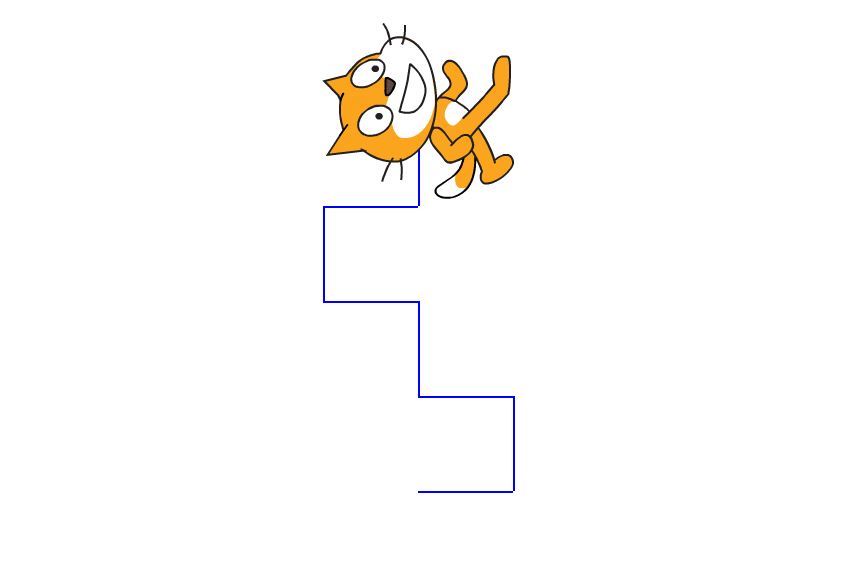
\includegraphics[width=0.7\textwidth]{ecran-11-eg1} 
\end{center}
qui a été réalisée à l'aide des éléments de programmation suivants : %Je veux réaliser cette figure.

\begin{minipage}{0.49\textwidth}
\begin{itemize}
  \item Quatre nouveaux blocs ont été définis : 
  \codeinline{monbloc1},  \codeinline{monbloc2},  \codeinline{monbloc3} et  \codeinline{monbloc4}.

\bigskip
  
  \item Lorsque le drapeau vert est cliqué, ces quatre blocs sont exécutés (une seule fois chacun).
  
\bigskip
  
  \item Malheureusement, les blocs ont été détachés et classés par ordre alphabétique !%j'ai oublié dans quel ordre je devais les placer afin de réaliser ma figure !
  
\end{itemize} 
\end{minipage}
\begin{minipage}{0.49\textwidth}
\begin{center}
\setscratch{scale=0.75}
\begin{scratch}
  \blockinit{quand \greenflag est cliqué}
  \blockmove{aller à x: \ovalnum{0} y: \ovalnum{-100}}
  \blockmove{s'orienter à \ovalnum{90}}
  \blockpen{effacer tout}
  \blockpen{stylo en position d'écriture}
  \blockspace[0.5]
  \blockmoreblocks{monbloc1}
  \blockspace[0.5]
  \blockmoreblocks{monbloc2}
  \blockspace[0.5]
  \blockmoreblocks{monbloc3}
  \blockspace[0.5]
  \blockmoreblocks{monbloc4}
\end{scratch}
\end{center} 
\end{minipage}

\medskip
\bigskip
\bigskip

Voici les définitions des quatre blocs :
\begin{center}
\setscratch{scale=0.75}
\begin{scratch}
\initmoreblocks{définir \namemoreblocks{monbloc1}}
  \blockmove{s'orienter à \ovalnum{90}}
  \blockmove{avancer de \ovalnum{50} pas}
  \blockmove{s'orienter à \ovalnum{0}}
  \blockmove{avancer de \ovalnum{50} pas}
\end{scratch}\quad
\begin{scratch}
\initmoreblocks{définir \namemoreblocks{monbloc2}}
  \blockmove{s'orienter à \ovalnum{-90}}
  \blockmove{avancer de \ovalnum{50} pas}
  \blockmove{ajouter \ovalnum{50} à y}
\end{scratch}\quad
\begin{scratch}
\initmoreblocks{définir \namemoreblocks{monbloc3}}
  \blockmove{ajouter \ovalnum{50} à x}
  \blockmove{tourner \turnleft{} de \ovalnum{90} degrés}
  \blockmove{avancer de \ovalnum{50} pas}
\end{scratch}\quad
\begin{scratch}
\initmoreblocks{définir \namemoreblocks{monbloc4}}
  \blockmove{avancer de \ovalnum{50} pas}
  \blockmove{tourner \turnright{} de \ovalnum{90} degrés}
  \blockmove{avancer de \ovalnum{50} pas}
\end{scratch}
\end{center} 




\bigskip

\textbf{Question.} Quel doit être l'ordre des blocs ?
Réponds sous la forme d'un entier à quatre chiffres. Par exemple, s'il faut exécuter \codeinline{monbloc2}, puis
\codeinline{monbloc3}, puis \codeinline{monbloc1}, puis \codeinline{monbloc4}, alors réponds 2314.

%\begin{solution}
%Réponse : 3241
%\end{solution}

\end{enigme}

\bigskip
\bigskip
\bigskip
\bigskip
\bigskip
\bigskip

\begin{enigme}

  Voici une nouvelle figure :
  \begin{center}
    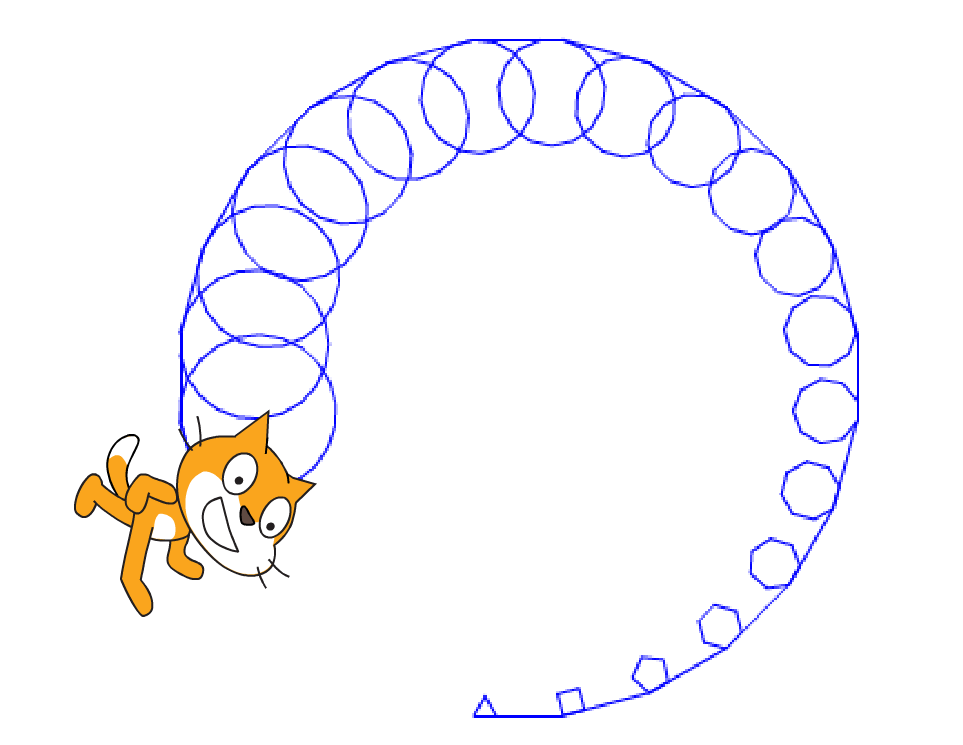
\includegraphics[width=0.56\textwidth]{ecran-11-eg2} 
  \end{center}
  réalisée par les éléments de programmation suivants : 

\begin{minipage}{0.49\textwidth}
\begin{itemize}
  \item Il est fait appel à un nouveau bloc \codeinline{monbloc(n)} dont les instructions dépendent d'un entier $n$.

\bigskip
  
  \item Lorsque le drapeau vert est cliqué, la variable $n$ est initialisée à une certaine valeur, puis une boucle utilise plusieurs fois \codeinline{monbloc}.
  
\bigskip
  
  \item Malheureusement, une donnée a été effacée, celle qui fixe l'initialisation de la variable $n$ !
\end{itemize} 
\end{minipage}
\begin{minipage}{0.49\textwidth}
\begin{center}
\setscratch{scale=0.6}
\begin{scratch}
  \blockinit{quand \greenflag est cliqué}
  \blockvariable{mettre \selectmenu{n} à \ovalnum{???}}
  \blockrepeat{répéter \ovalnum{20} fois}{
    \blockmoreblocks{monbloc \ovalvariable{n}}
    \blockmove{avancer de \ovalnum{40} pas}
    \blockmove{tourner \turnleft{} de \ovalnum{15} degrés}
    \blockvariable{ajouter \ovalnum{1} à \selectmenu{n}}
  }
%  \blockspace
\end{scratch}

\bigskip

\begin{scratch}
\initmoreblocks{définir \namemoreblocks{monbloc} \ovalmoreblocks{n}}
  \blockrepeat{répéter \ovalmoreblocks{n} fois}{
    \blockmove{avancer de \ovalnum{10} pas}
    \blockmove{tourner \turnleft{} de \ovaloperator{\ovalnum{360} / \ovalmoreblocks{n}} degrés}
  }
\end{scratch}
\end{center} 
\end{minipage}



\bigskip

\textbf{Question.} Par quelle valeur faut-il remplacer les \og{}???\fg{} afin d'obtenir en fin d'exécution le dessin voulu ?

%\begin{solution}
%Réponse $n=3$ car \codeinline{monbloc(n)} dessine un polygone à $n$ côtés.
%\end{solution}

\end{enigme}

\bigskip

\begin{enigme}

Scratch souhaite dessiner cet arbre 
\begin{center}
  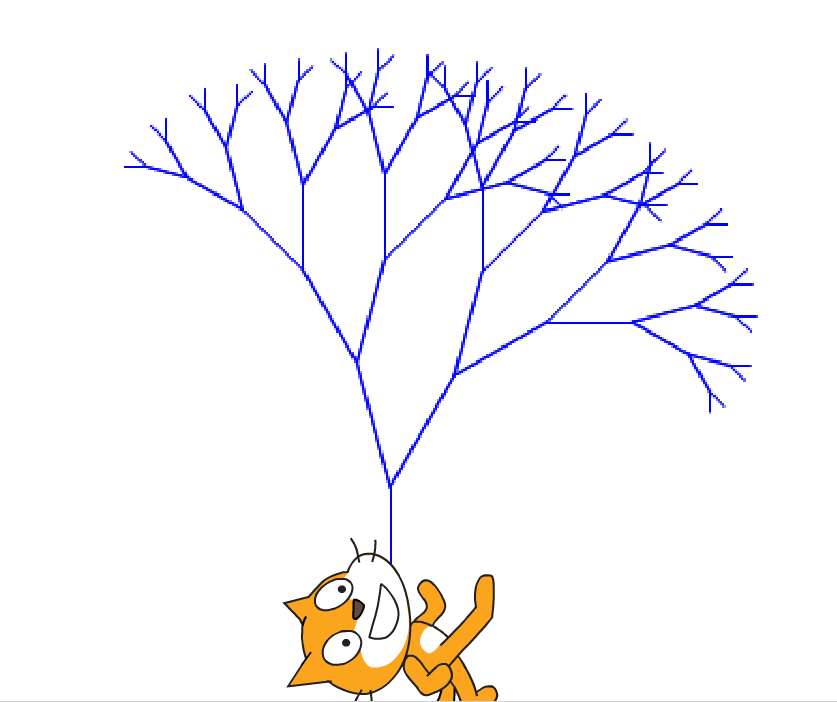
\includegraphics[width=0.55\textwidth]{ecran-11-eg3} 
\end{center}
avec les éléments de programmation suivants : %Voici le programme proposé !

\begin{center}
\setscratch{scale=0.7}
\begin{scratch}
  \blockinit{quand \greenflag est cliqué}

  \blockmove{aller à x: \ovalnum{0} y: \ovalnum{-150}}
  \blockmove{s'orienter à \ovalnum{0}}
  \blockpen{effacer tout}
  \blockpen{stylo en position d'écriture}

  \blockmoreblocks{branche \ovalnum{???}}
\end{scratch}\qquad\qquad
\begin{scratch}
  \initmoreblocks{définir \namemoreblocks{branche} \ovalmoreblocks{n}}
  \blockif{si \booloperator{\ovalmoreblocks{n} > \ovalnum{0}} alors  }
  {
    \blockmove{avancer de \ovaloperator{\ovalmoreblocks{n} * \ovalnum{10}} pas}
    \blockmove{tourner \turnleft{} de \ovalnum{15} degrés}
    \blockmoreblocks{branche \ovaloperator{\ovalmoreblocks{n} - \ovalnum{1}}}
    \blockmove{tourner \turnright{} de \ovalnum{45} degrés}
    \blockmoreblocks{branche \ovaloperator{\ovalmoreblocks{n} - \ovalnum{1}}}
    \blockmove{tourner \turnleft{} de \ovalnum{30} degrés}
    \blockmove{avancer de \ovaloperator{\ovalmoreblocks{n} * \ovalnum{-10}} pas}
  }
\end{scratch}
\end{center}

\begin{itemize}
  \item Il semble que le programmeur soit devenu fou, car dans l'écriture du bloc \codeinline{branche(n)}, le programme fait appel
au bloc \codeinline{branche} lui-même à travers l'instruction \codeinline{branche(n-1)}.

  \item Et pourtant cela fonctionne !
  
   \item Par contre, le programmeur a oublié de préciser la valeur (notée \og{}???\fg{} ci-dessus) avec laquelle est appelé le bloc \codeinline{branche} .
\end{itemize}


\bigskip

\textbf{Question.} Par quelle valeur faut-il remplacer les \og{}???\fg{} afin d'obtenir en fin d’exécution le dessin voulu ?


%\begin{solution}
%Réponse $n=7$.
%\end{solution}

\end{enigme}

\end{document}

